\chapter{Eredmények}
\pagestyle{headings}

\section{Grafit-modell}
\subsection{Potenciáltérképezések}
Mint korábban említettem már, a pásztázó elektrokémiai mikroszkópiában általában egy céltárgy felszínét vizsgáljuk vagy az azon lejátszódó folyamatról szeretnénk információhoz jutni. Először egy jól ismert rendszert vizsgáltam meg, az előzőekben részletesebben jellemzett epoxi gyantába fogott grafit elektródpárt. A céltárgyat 2000 mV-al pozítivan polarizáltam, katódosan és anódosan egymáshoz képest. A feltérképezett katód környezetében hidrogénion redukciójára vagyis lokális pH növekedésre, az anódos oldalon pedig oxigén gáz fejlődésre számíthatunk, a következő egyenletek szerint:

K(-): 2H$^+$ + 2e$^-$ $\longrightarrow$ H$_2$ (redukció)

A(+):  2OH$^-$ $\longrightarrow$ 0,5 O$_2$ + H$_2$O + 2e$^-$ (oxidáció)

A mikroméretű referenciaelektróddal készített pásztázások horizontális potenciáltérképeit a (\ref{fig:horizontális}. ábra [E,F]), a vertikálisat pedig az (\ref{fig:vertikális}. ábra [C]) láthatjuk. A várakozásnak megfelelő eredményeket kaptam, hiszen mind a vertikális mind pedig a horizontális képeken, -5 mV eltéréssel, azonos potenciáltartományba esnek a mérések eredményei. Továbbá jól látható, hogy az elektródpár tagjai a polarizáció hatására katódként (-295 mV körüli átlagérték) és anódként (-265 mV körüli átlagérték) viselkedtek, ahogy azt elvártuk. Így az eredményekből látható, hogy a tanulmányozott rendszer ténylegesen állandó, jól jellemezhető és a módszer, amit használtam, alkalmazható a potenciáltérképezésre. 

\subsection{Elektromos mező és az áramsűrűség}
A \emph{Módszerek} című fejezetben említettek szerint elvégeztem a számolásokat, deriválást és így ábrázoltam vektorosan az elektromos mezőt, ami a (\ref{fig:field_gh}. ábra) és az (\ref{fig:field_v}. ábra [C]) láthatóak a grafit céltárgy esetében. Ezen belül az 5.4-es ábra (E) és (F) a horizontális pásztázások eredményei, az 5.5-ös ábra (C) képe pedig a vertikális. A Z tengelyen nézve az anód esetében az áramvektorok az oxidáció következtében a síkből kifelé mutatnak, a katódnál a redukció miatt pedig a síkba mutatnak a vektorok. Az X-Y síkon pedig az anódból a katód felé irányulnak a vetorok.  

Hasonlóan, az előző fejezetben leírtak alapján, elkészítettem az áramsűrűség térképét a Z irányú komponens szerint, a horizontális pásztázásra. Szakirodalomak alapján elmondhatjuk, hogy az anódos áramsűrűség pozitív értéket, a katódos pedig negatívat ad \cite{bastos2016preliminary}. Jól látható az (\ref{fig:áramsűrűség}. ábra [C]) képen, hogy a katód helyén (piros színnel jelölt) és környezetében negatív értékeket kaptam, a katód esetében (kék színnel jelölt) pedig pozitív értékeket, ahogy vártuk. A zölddel jelölt részen 0-nak tekinthető az áramerősség. Továbbá megfigyelhetjuk, hogy körülbelül szimmetrikusnak mondható a katód és anód régiójában áramerősség és ez távolódva a helyüktől csökkenést mutat. Ez a térkép az elektromos mezőével mutat hasonlóságot, mivel az előzőleg már említett (\ref{fig:nabla}. egyenlet) szerint a két érték között egyenes arányosság van \cite{{isaacs1981scanning},{bastos2017application}}. Az eredmények a várakozással egyeztek ezen esetben is, így ezt a galvánpár esetében is alkalmaztam.

\section{Vas-cink galvánpár korrózió vizsgálata}
\subsection{Potenciáltérképezések}
Az előző alfejezetben bemutatott grafit céltárgy után egy vas-cink galvánpárból készült céltárgyat tanulmányoztam, melyet a \emph{Módszerek} fejezetben jellemeztem részletesebben. Ez egy sokszor vizsgált és előforduló rendszer, mivel a vas ötvözeteit, illetve magát a vasat is, számos esetben vonjuk be a jobb korrózióállóság miatt cinkréteggel. Ezt a technikát a hétköznapi életben horganyzásnak hívjuk, ezzel a módszerrel jelentős mértékben csökkenthető a védett fém korróziója. Ez annak tulajdonítható, hogy a cink tölti be az \emph{Irodalom} fejezetben említett áldozati anód szerepét a galvanikus kapcsolat során, mivel az egyik legaktívabb fémek közé sorolható. Tehát a cink oxidálódik a védett fém, vagyis a vas helyett. Ezzel egyidőben a vason redukció zajlik, viszont vaskioldódás nélkül. Ennek a folyamatnak is a lényege a hidrogénion redukció, így ahogy az előző alfejezetben jellemzett grafit katód esetén is, lokális pH növekedésre számíthatunk jelen esetben is. A cink anódon a következő reakciók játszódnak le:

2 Zn $\longrightarrow$ 2 Zn$^{2+}$ + 4e$^-$ 

Zn$^{2+}$ + nH$_2$O $\longrightarrow$ Zn(OH)$_{n2-n}$ + nH$^+$


A vas katódon pedig a következő reakciók mennek végbe:

2H$^+$ + 2e$^-$ $\longrightarrow$ H$_2$

O$_2$ + 4H$_2$O + 4e$^-$ $\longrightarrow$ 2H$_2$O + 4OH$^-$

A vizsgálatok potenciáltérképei az (\ref{fig:horizontális}. ábra) és (\ref{fig:vertikális}. ábra) láthatóak. Ebben az esetben külön pásztáztam, a katód (\ref{fig:horizontális}. ábra [A,B]) és az anód (\ref{fig:horizontális}. ábra [C,D]) felületét a grafittal ellentétben. A felület homogén, vagyis a vas egész felülete katódként viselkedett a cellában a mérés alatt, ezzel alátámasztva, hogy a cinkelektród működött csak anódként. Ezt bizonyítja az eltérő mért potenciálértékek is, vagyis anódra jellemzően nagyobb, a cinknél -230 mV, körüli érték, és a vas esetében kisebb, -275 mV körüli érték, hasonlóan a grafit modell elvéhez. Illetve leolvasható, hogy a potenciáltartomány értékei a 3-3 pásztázásnak körülbelül azonos minimum és maximum értéket követnek itt is. A vas vertikális potenciálképénél (\ref{fig:vertikális}. ábra [A]) látható egy szélesebb tartomány, mint a horizontális képeknél. Ez valószínűleg annak tulajdonítható, hogy a grafittól eltérően, ez a korróziós folyamat időben változó. A vertikális pásztázása és a horizontálisak között több idő telhetett el, ami során a reakció előre haladt már, így kaptam az eltérő értékeket a tartományra. Ha szétkapcsolnánk a cellát, a vas felületén lokális anód és katód alakulna ki, vagyis elvesztené a cink anódos védelmét. Láthatóvá válnának a felületen sárgás-barnás elszíneződések, vagyis a rozsdásodás folyamata beindulna. Ezen részek anódként viselkednek, nem tudnánk itt katódos aktivitást kimutatni. 

\subsection{Elektromos mező és az áramsűrűség}

Az előző fejezetben leírtak szerint ábrázoltam vektorosan ebben az esetben is az elektromos mezőt, ami az (\ref{fig:field_h}. ábra [A-D]) és az (\ref{fig:field_v}. ábra [A,B]) láthatóak a vas-cink galvánpár esetében. Ezen belül az 5.3-as ábra (A) és (B) a vas katód, (C) és (D) a cink anód horizontális pásztázások eredményei, az 5.5-ös ábra (A) képe a vas katód, (B) képe pedig a cink anód a vertikális eredményei. A Z tengely szerint nézve a vas katód esetében az áramvektorok a síkből kifelé mutatnak, mivel az előző alfejezetben leírtak szerint lejátszódó redukció miatt. A cink anódnál pedig, a szintén leírt egyenletek szerint lejátszódó oxidáció miatt, a síkba mutatnak a vektorok. Az X-Y síkon pedig az anódból a katód felé irányulnak a vetorok, a grafit modell rendszer elvéhez hasonlóan, azonban mivel külön készítettem a mérést az anódról és katódról, így nem látható ez egyertelműen.  

Hasonlóan, jártam el a galvánpár esetben is, mikor elkészítettem az áramsűrűség térképét a Z irányú komponens szerint, a horizontális pásztázásokra. A grafithoz hasonlóan, hogy az anódos áramsűrűség pozitív értéket, a katódos pedig negatív értéket ad. Megfigyelhető az (\ref{fig:áramsűrűség}. ábra [A]) képén, hogy az vas katód lokális környezetében negatív értékeket kaptam. Ugyanezen ábra (B) képén a cink anód esetében pedig pozitív értékeket, ahogy vártuk. A zölddel jelölt részen 0-nak tekinthető az áramerősség értéke. Ezen céltárgynál is elmondhatjuk, hogy körülbelül szimmetrikus a katód és anód régiójában áramerősség és ez távolódva a helyüktől csökkenést mutat. Illetve a térkép itt is hasonlóságot mutat az elektromos mezőével.

%\includegraphics[trim = 10mm 40mm 0mm 40mm, clip, width=0.4\textwidth, angle=-90]{img/mg_metal/liquid_uncoupled.eps} \includegraphics[trim = 10mm 40mm 0mm 40mm, clip, width=0.4\textwidth, angle=-90]{img/mg_metal/solid_uncoupled.eps}

\begin{figure}
\centering
\includegraphics[width=0.3\textwidth, angle=-90]{img/mérések/Fe_h_100.eps}\includegraphics[width=0.3\textwidth, angle=-90]{img/mérések/Fe_h_500.eps}

\includegraphics[width=0.3\textwidth, angle=-90]{img/mérések/Zn_h_100.eps}\includegraphics[width=0.3\textwidth, angle=-90]{img/mérések/Zn_h_500.eps}

\includegraphics[width=0.3\textwidth, angle=-90]{img/mérések/grafit_h_100.eps}
\includegraphics[width=0.3\textwidth, angle=-90]{img/mérések/grafit_h_300.eps}

\caption{Az említett céltárgyakról készült horizontális potenciáltérképek:
(A) és (B) a vas katód 100$\upmu$m és 500$\upmu$m magasságban, (C) és (D) a cink anód 100$\upmu$m és 500$\upmu$m magasságban és (E) és (F) a grafit katódja és anódja 100$\upmu$m és 300$\upmu$m magasságban mérve}
\label{fig:horizontális}
\end{figure}


\begin{figure}
\centering
\includegraphics[width=0.3\textwidth, angle=-90]{img/mérések/Fe_v.eps}
\includegraphics[width=0.3\textwidth, angle=-90]{img/mérések/Zn_v.eps}
\includegraphics[width=0.3\textwidth, angle=-90]{img/mérések/grafit_v.eps}


\caption{Az említett céltárgyakról készült vertikális potenciáltérképek:
(A) a vas katód, (B) a cink anód és (C) a grafit katódja és anódja}
\label{fig:vertikális}
\end{figure}

\begin{figure}
\centering
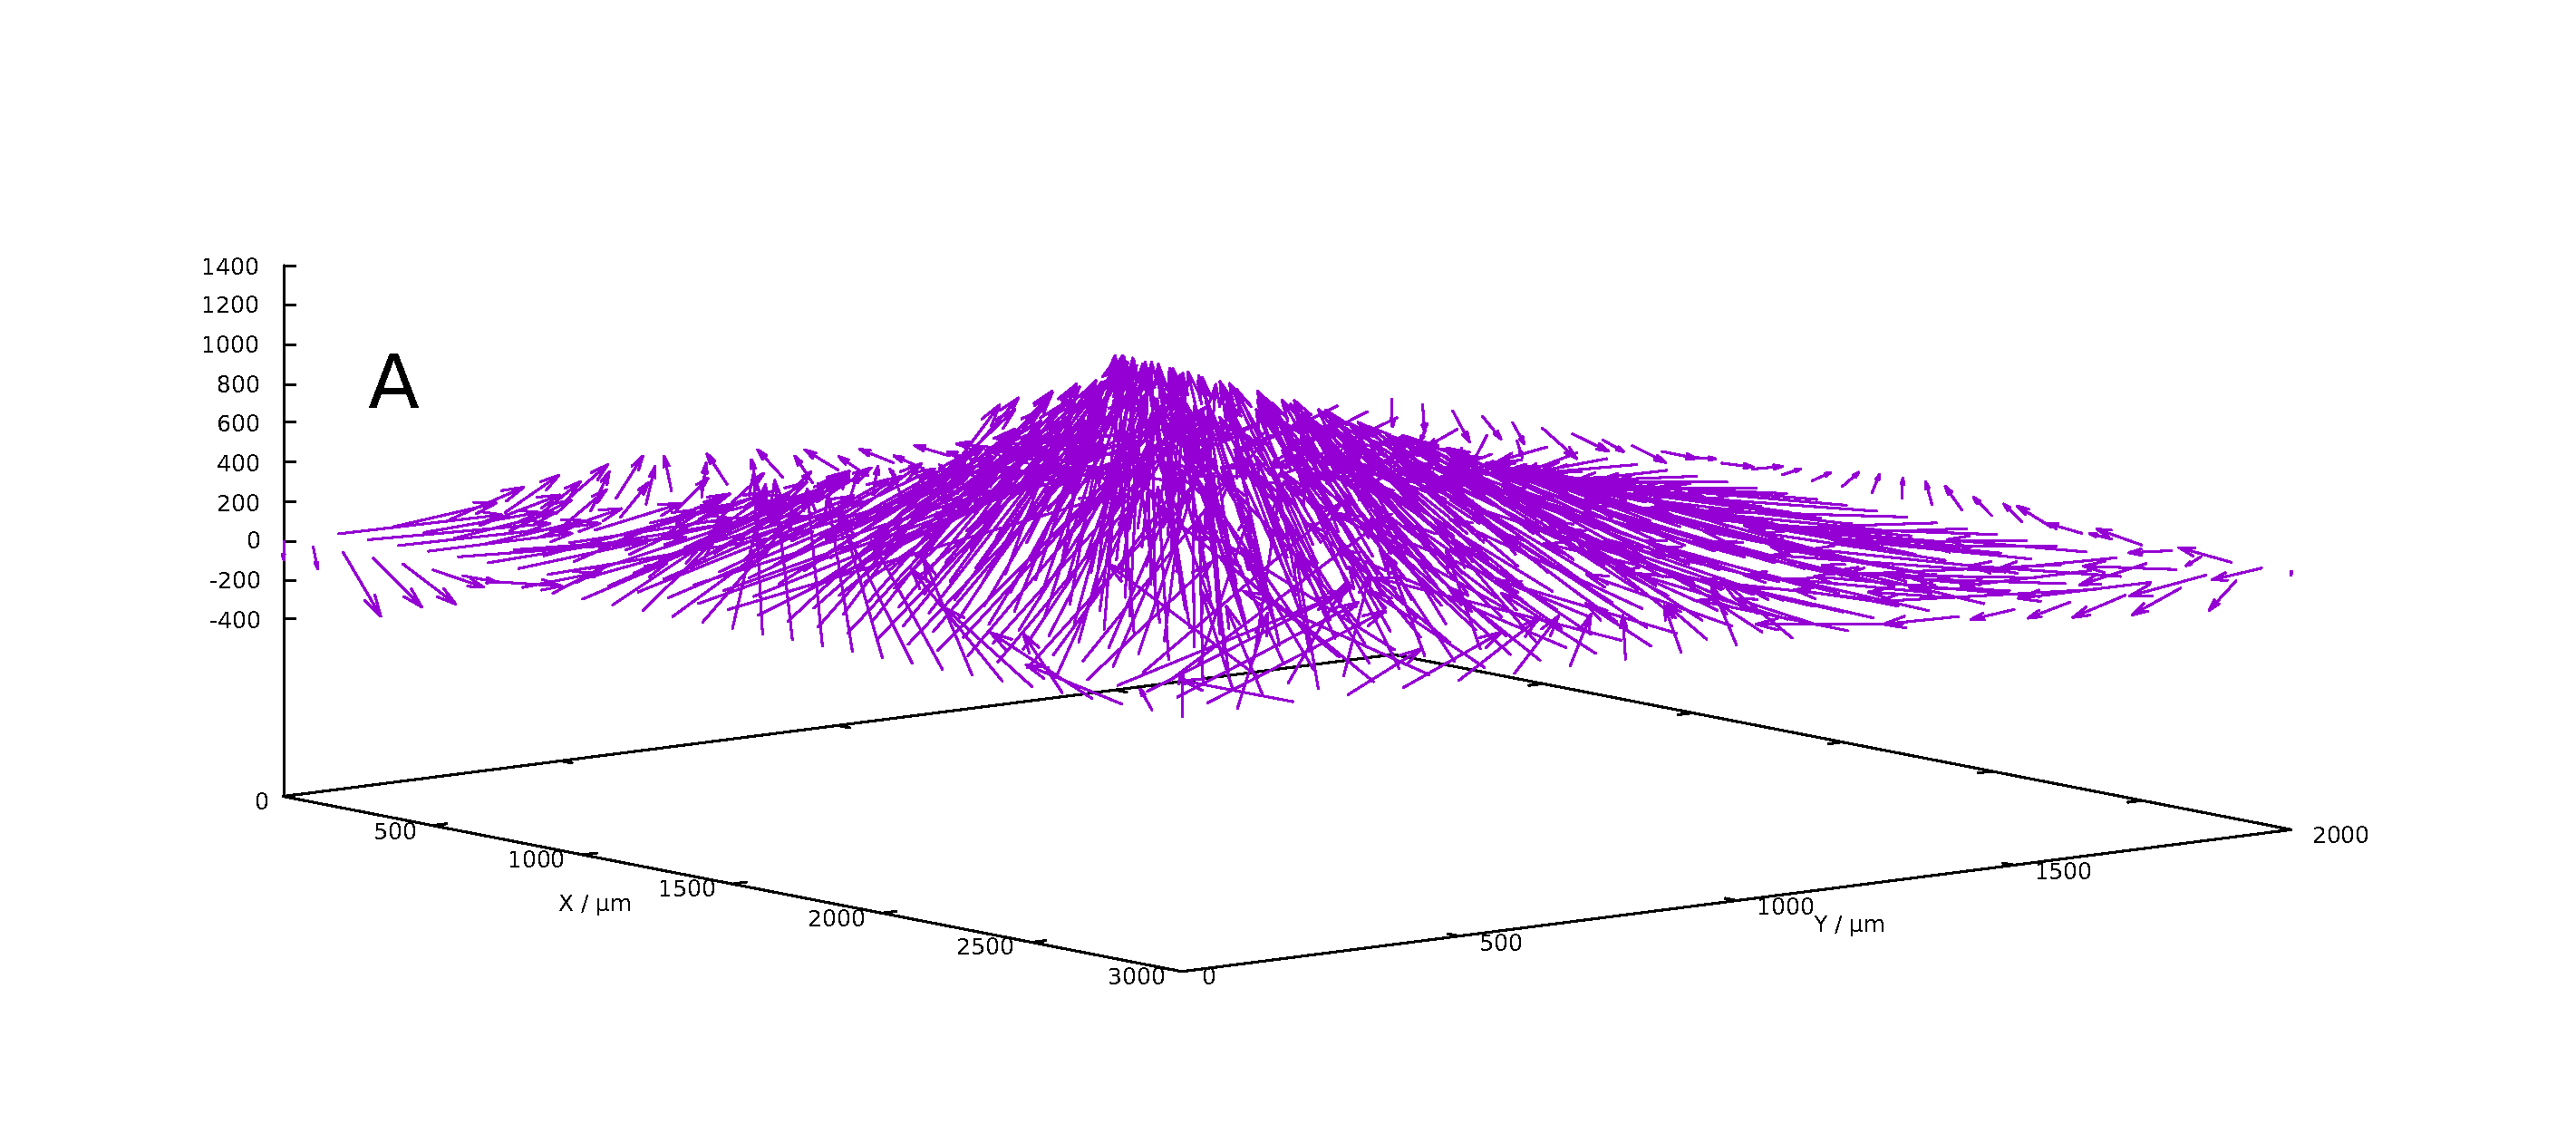
\includegraphics[width=1\textwidth]{img/mérések/Fe_h100.pdf}
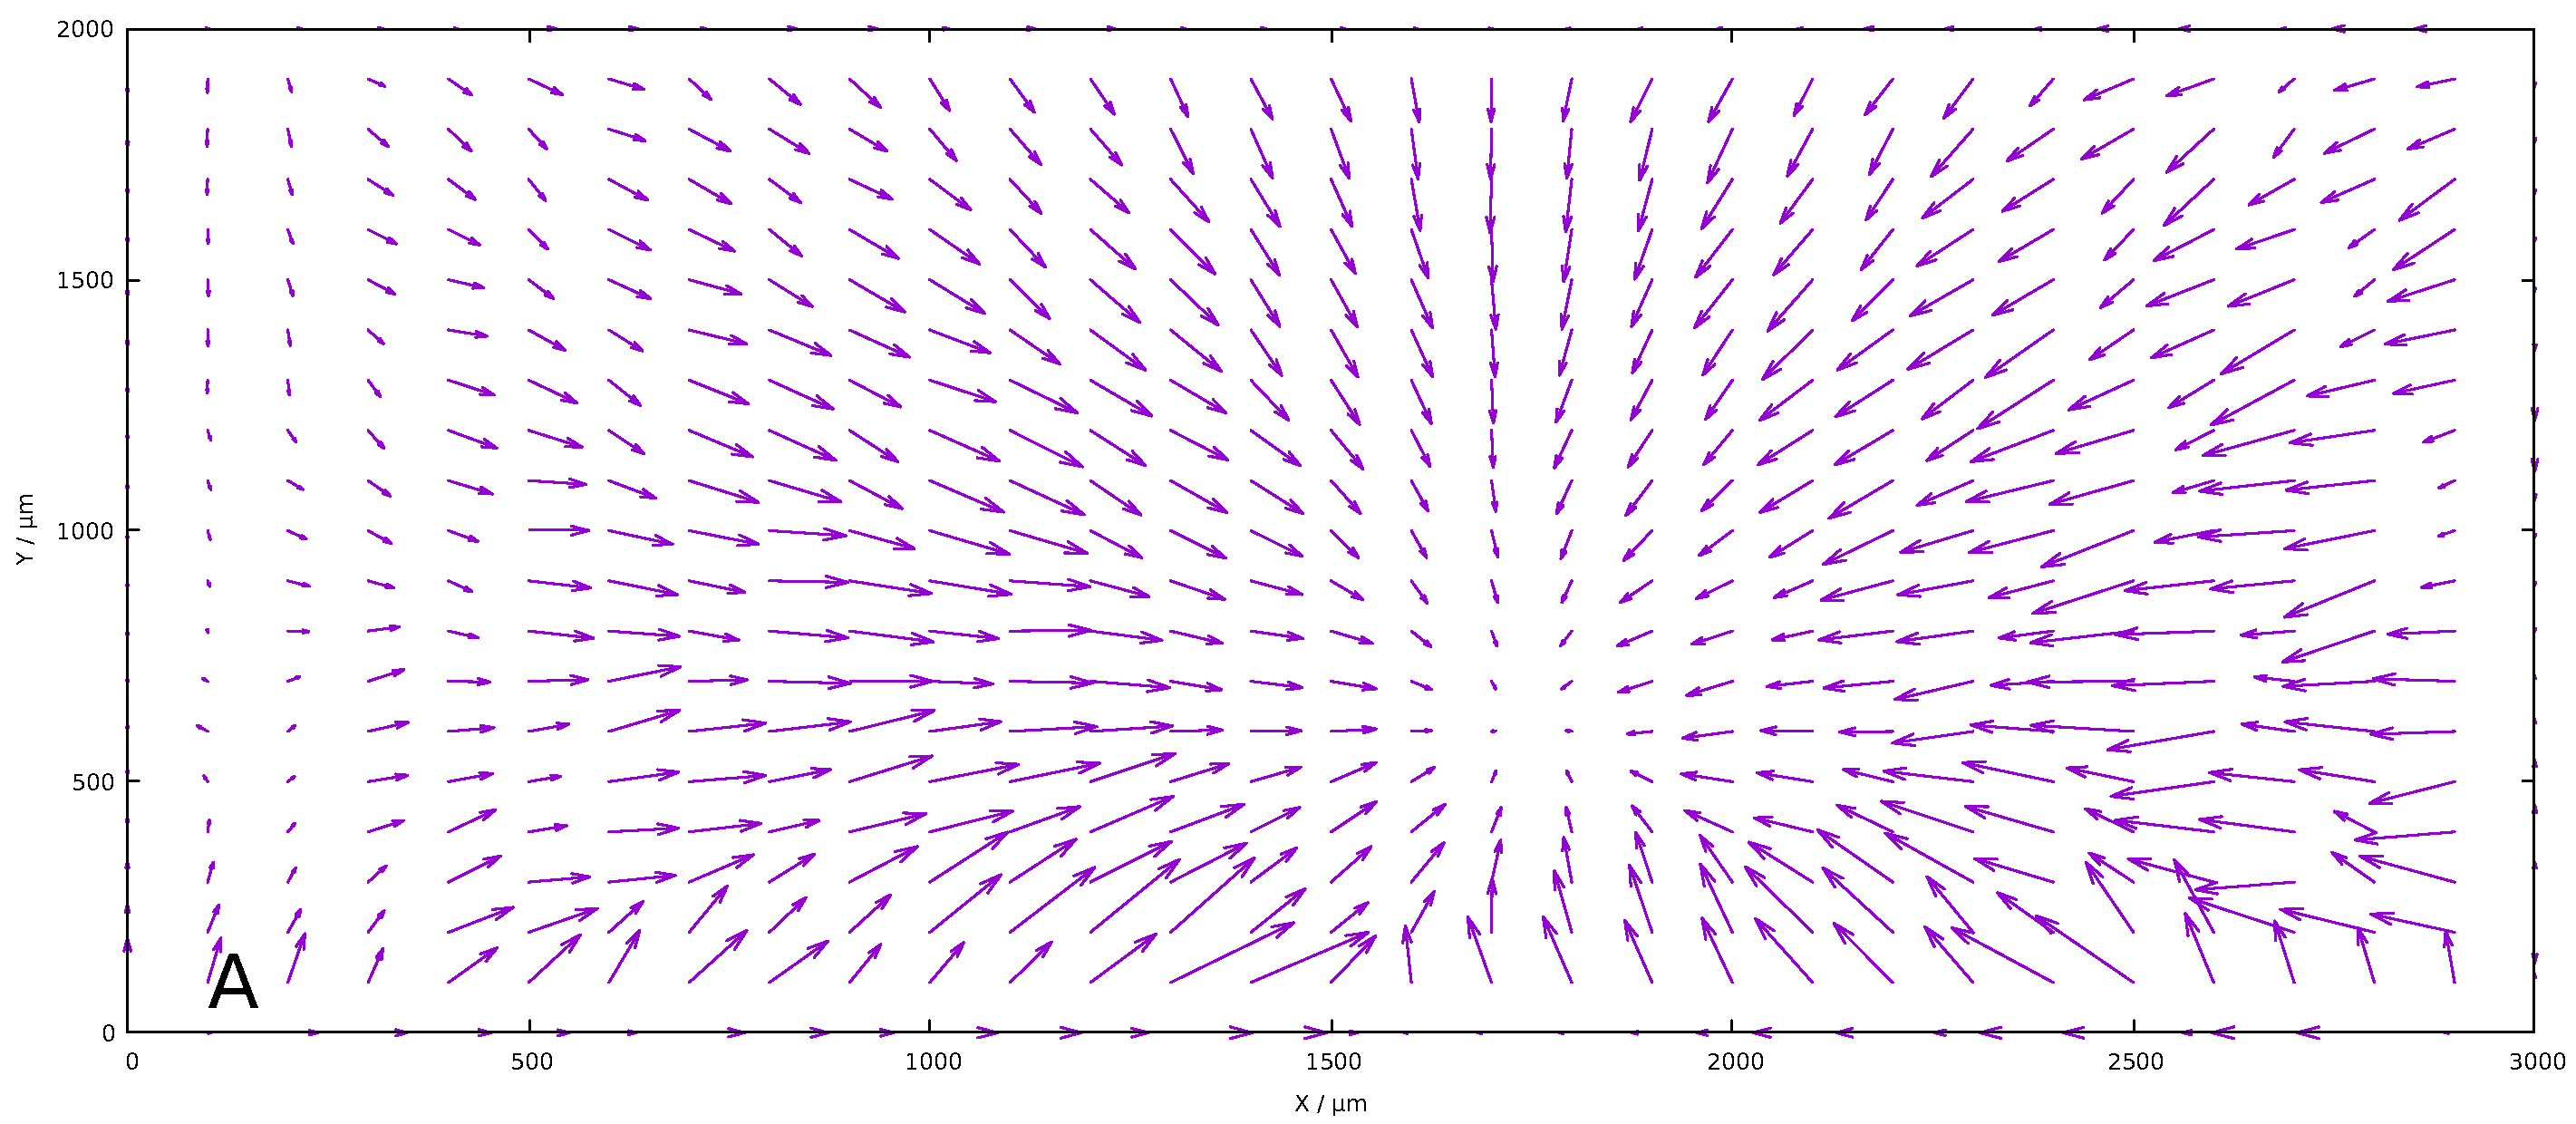
\includegraphics[width=0.8\textwidth]{img/mérések/Fe1_h100.pdf}

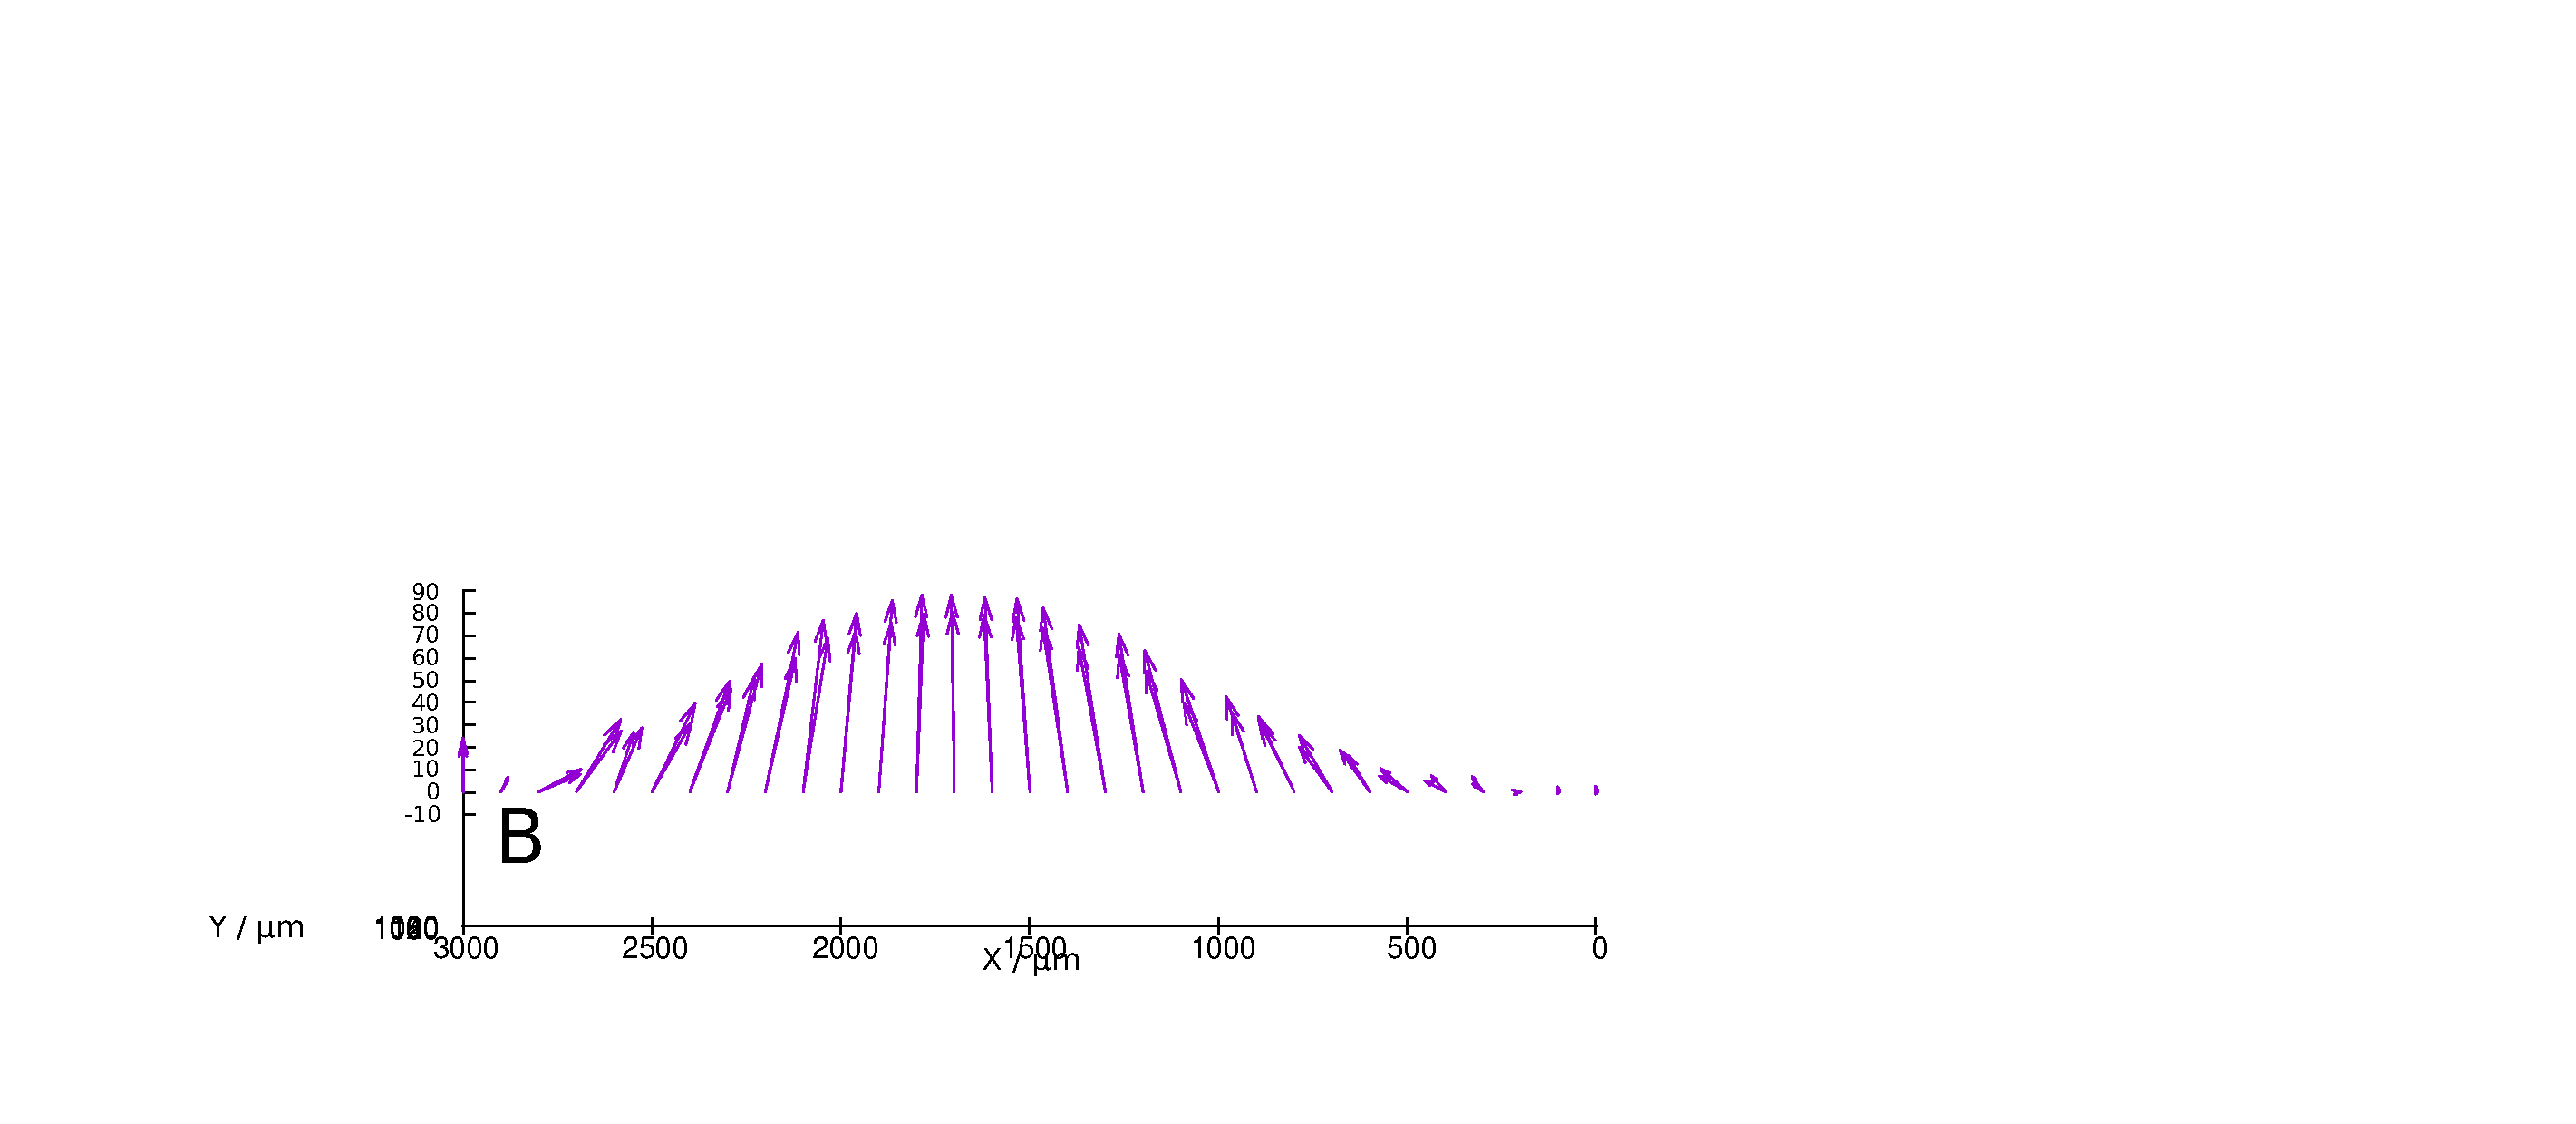
\includegraphics[width=1\textwidth]{img/mérések/Zn_h100.pdf}
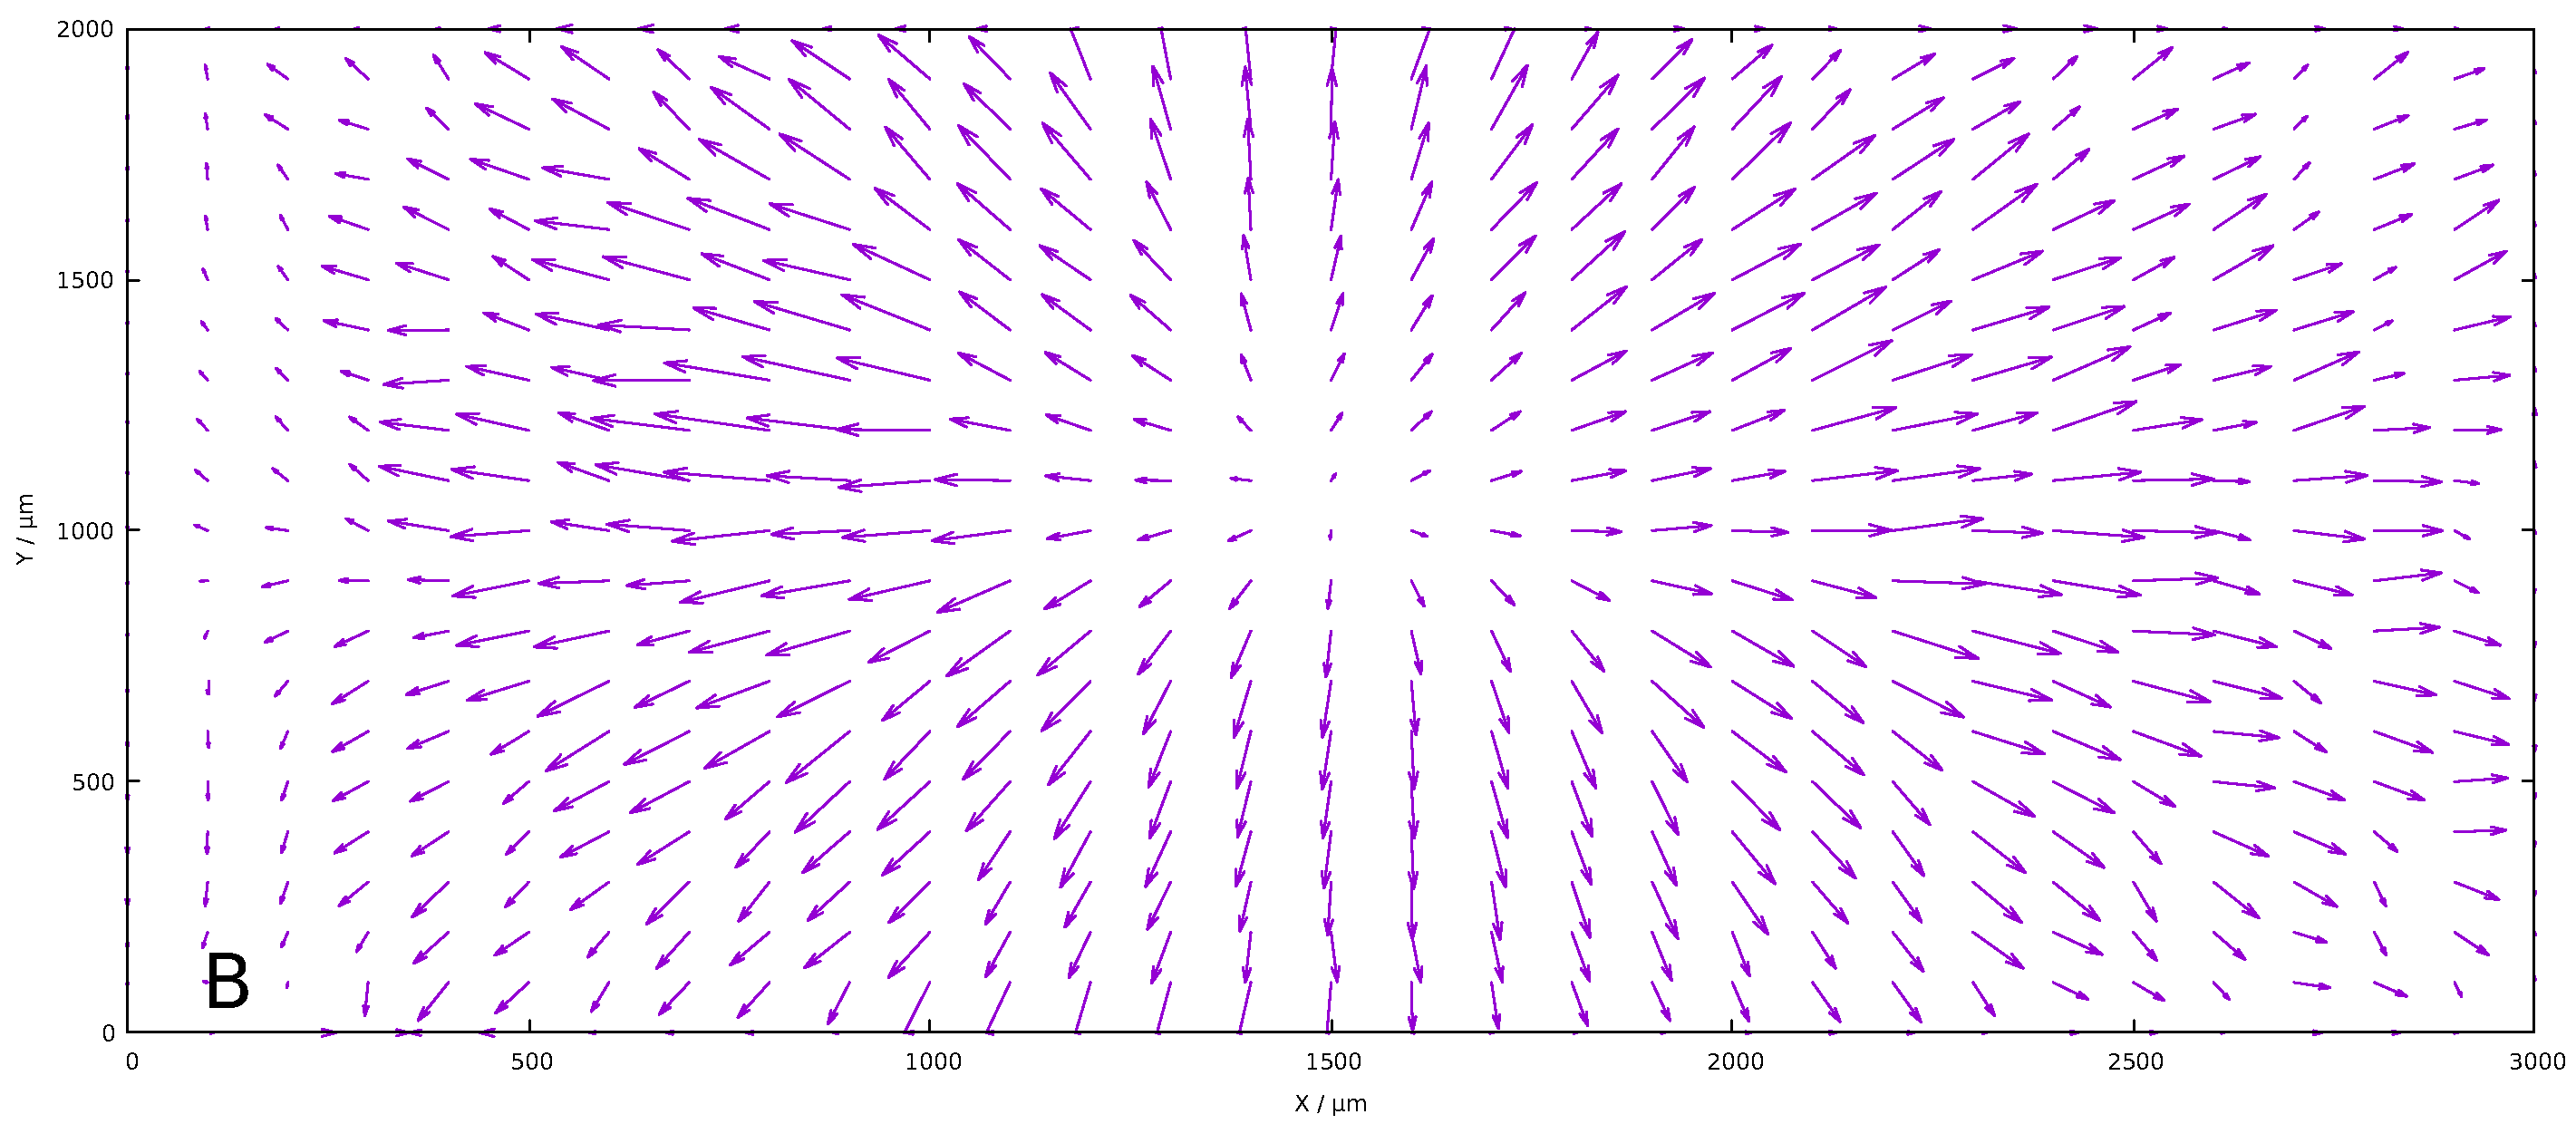
\includegraphics[width=0.8\textwidth]{img/mérések/Zn1_h100.pdf}

\caption{Az említett cink-vas pár céltárgyról készült horizontális elektromos mező térképek:
(A) a vas katód és (B) a cink anód 100$\upmu$m magasságban mérve}
\label{fig:field_h}
\end{figure}

\begin{figure}
\centering
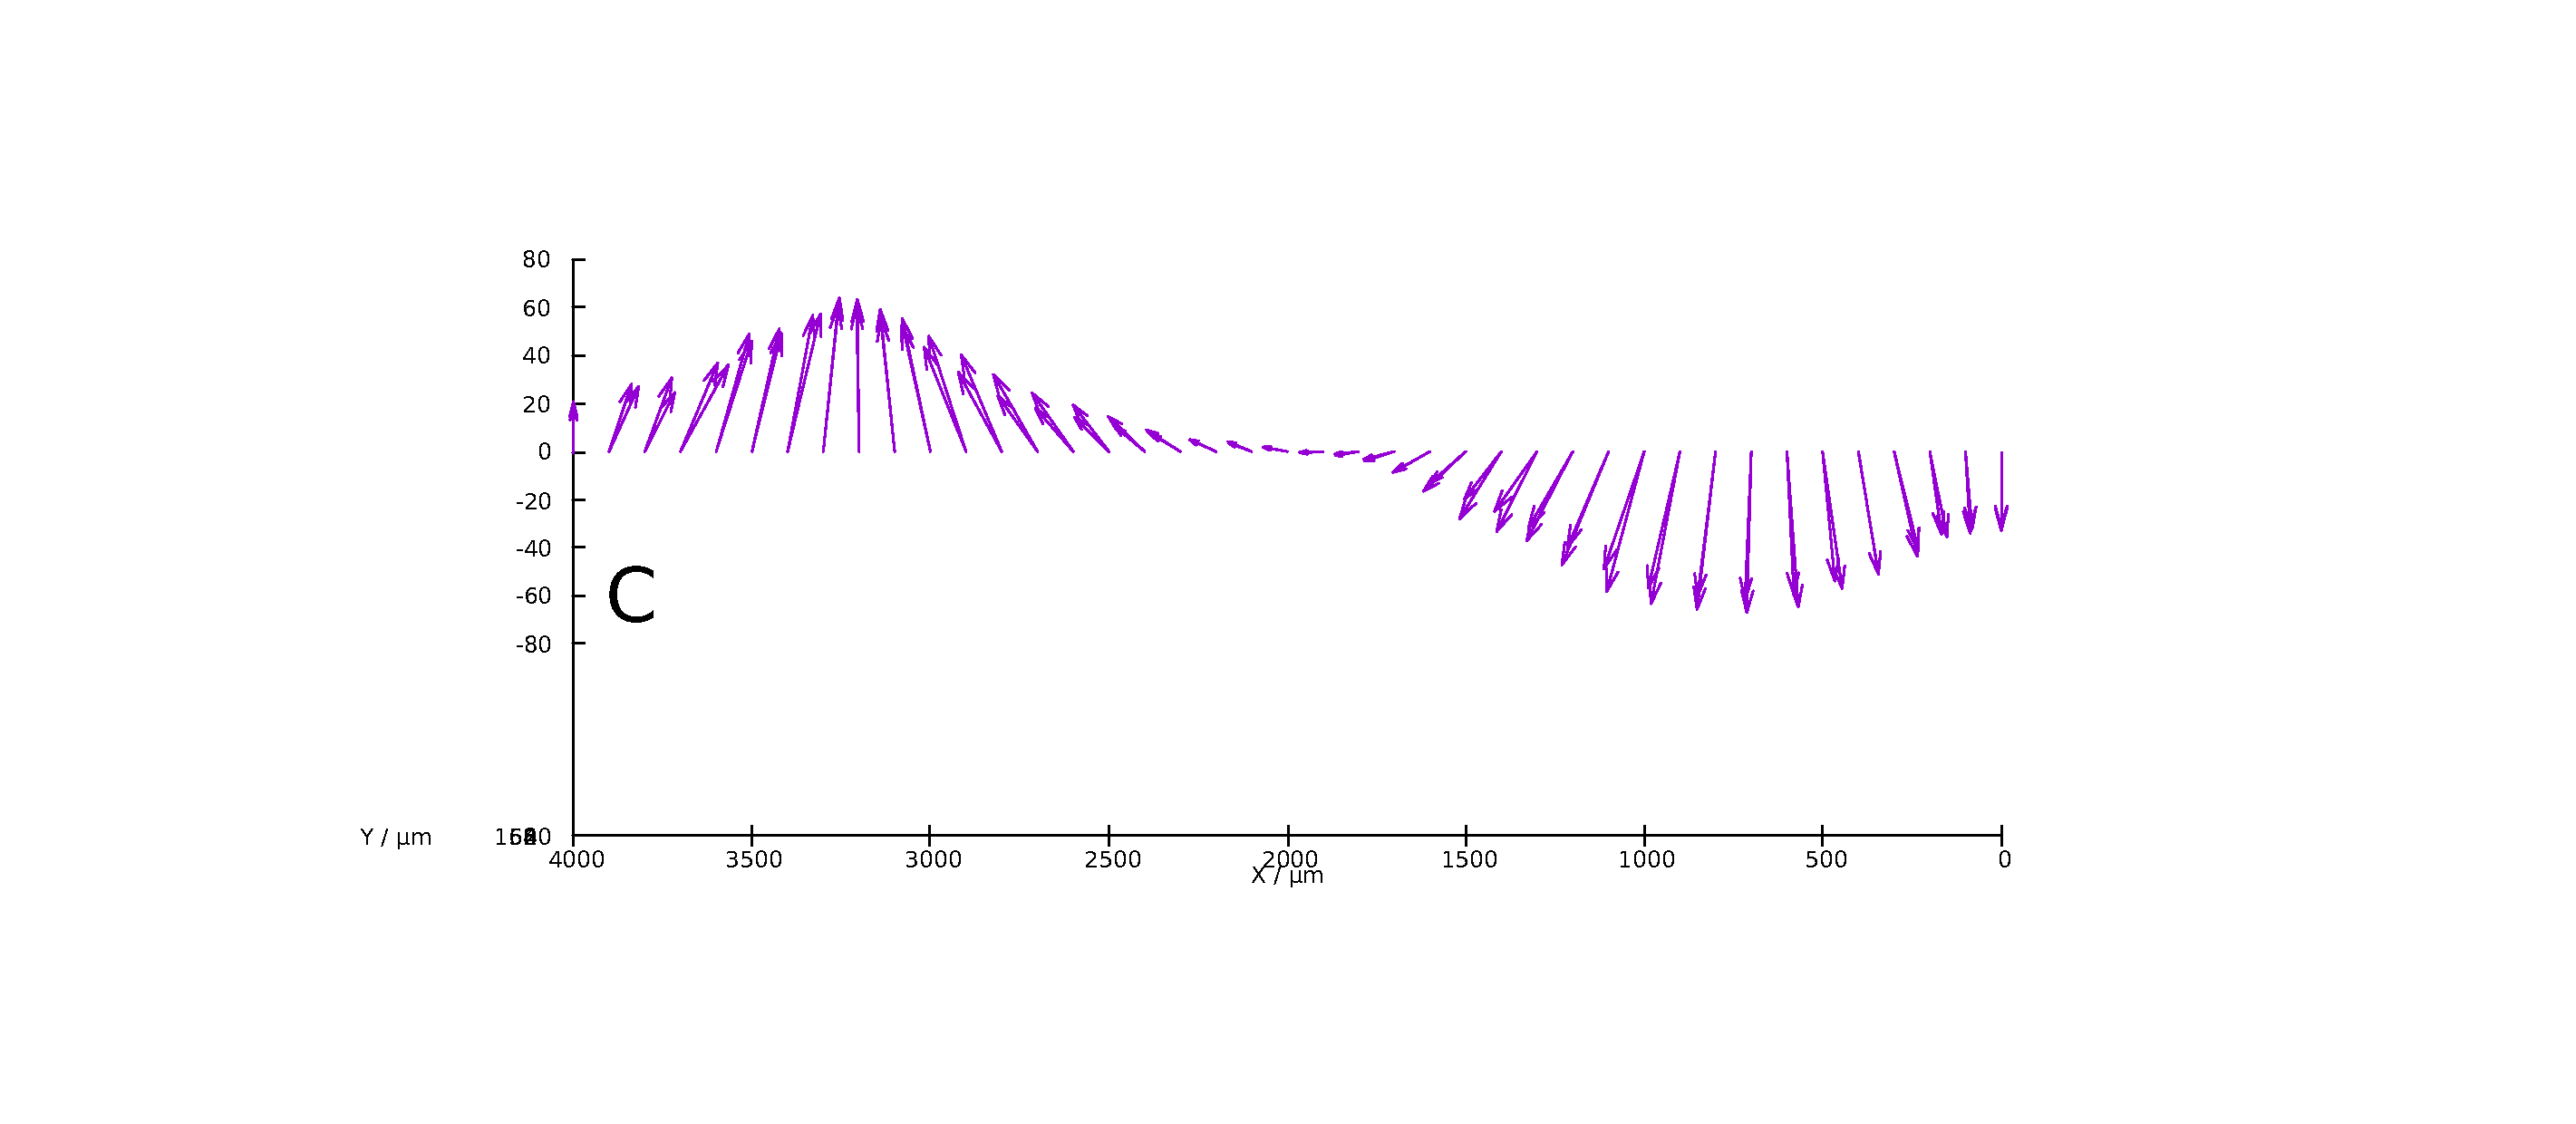
\includegraphics[width=1\textwidth]{img/mérések/grafit_h100.pdf}
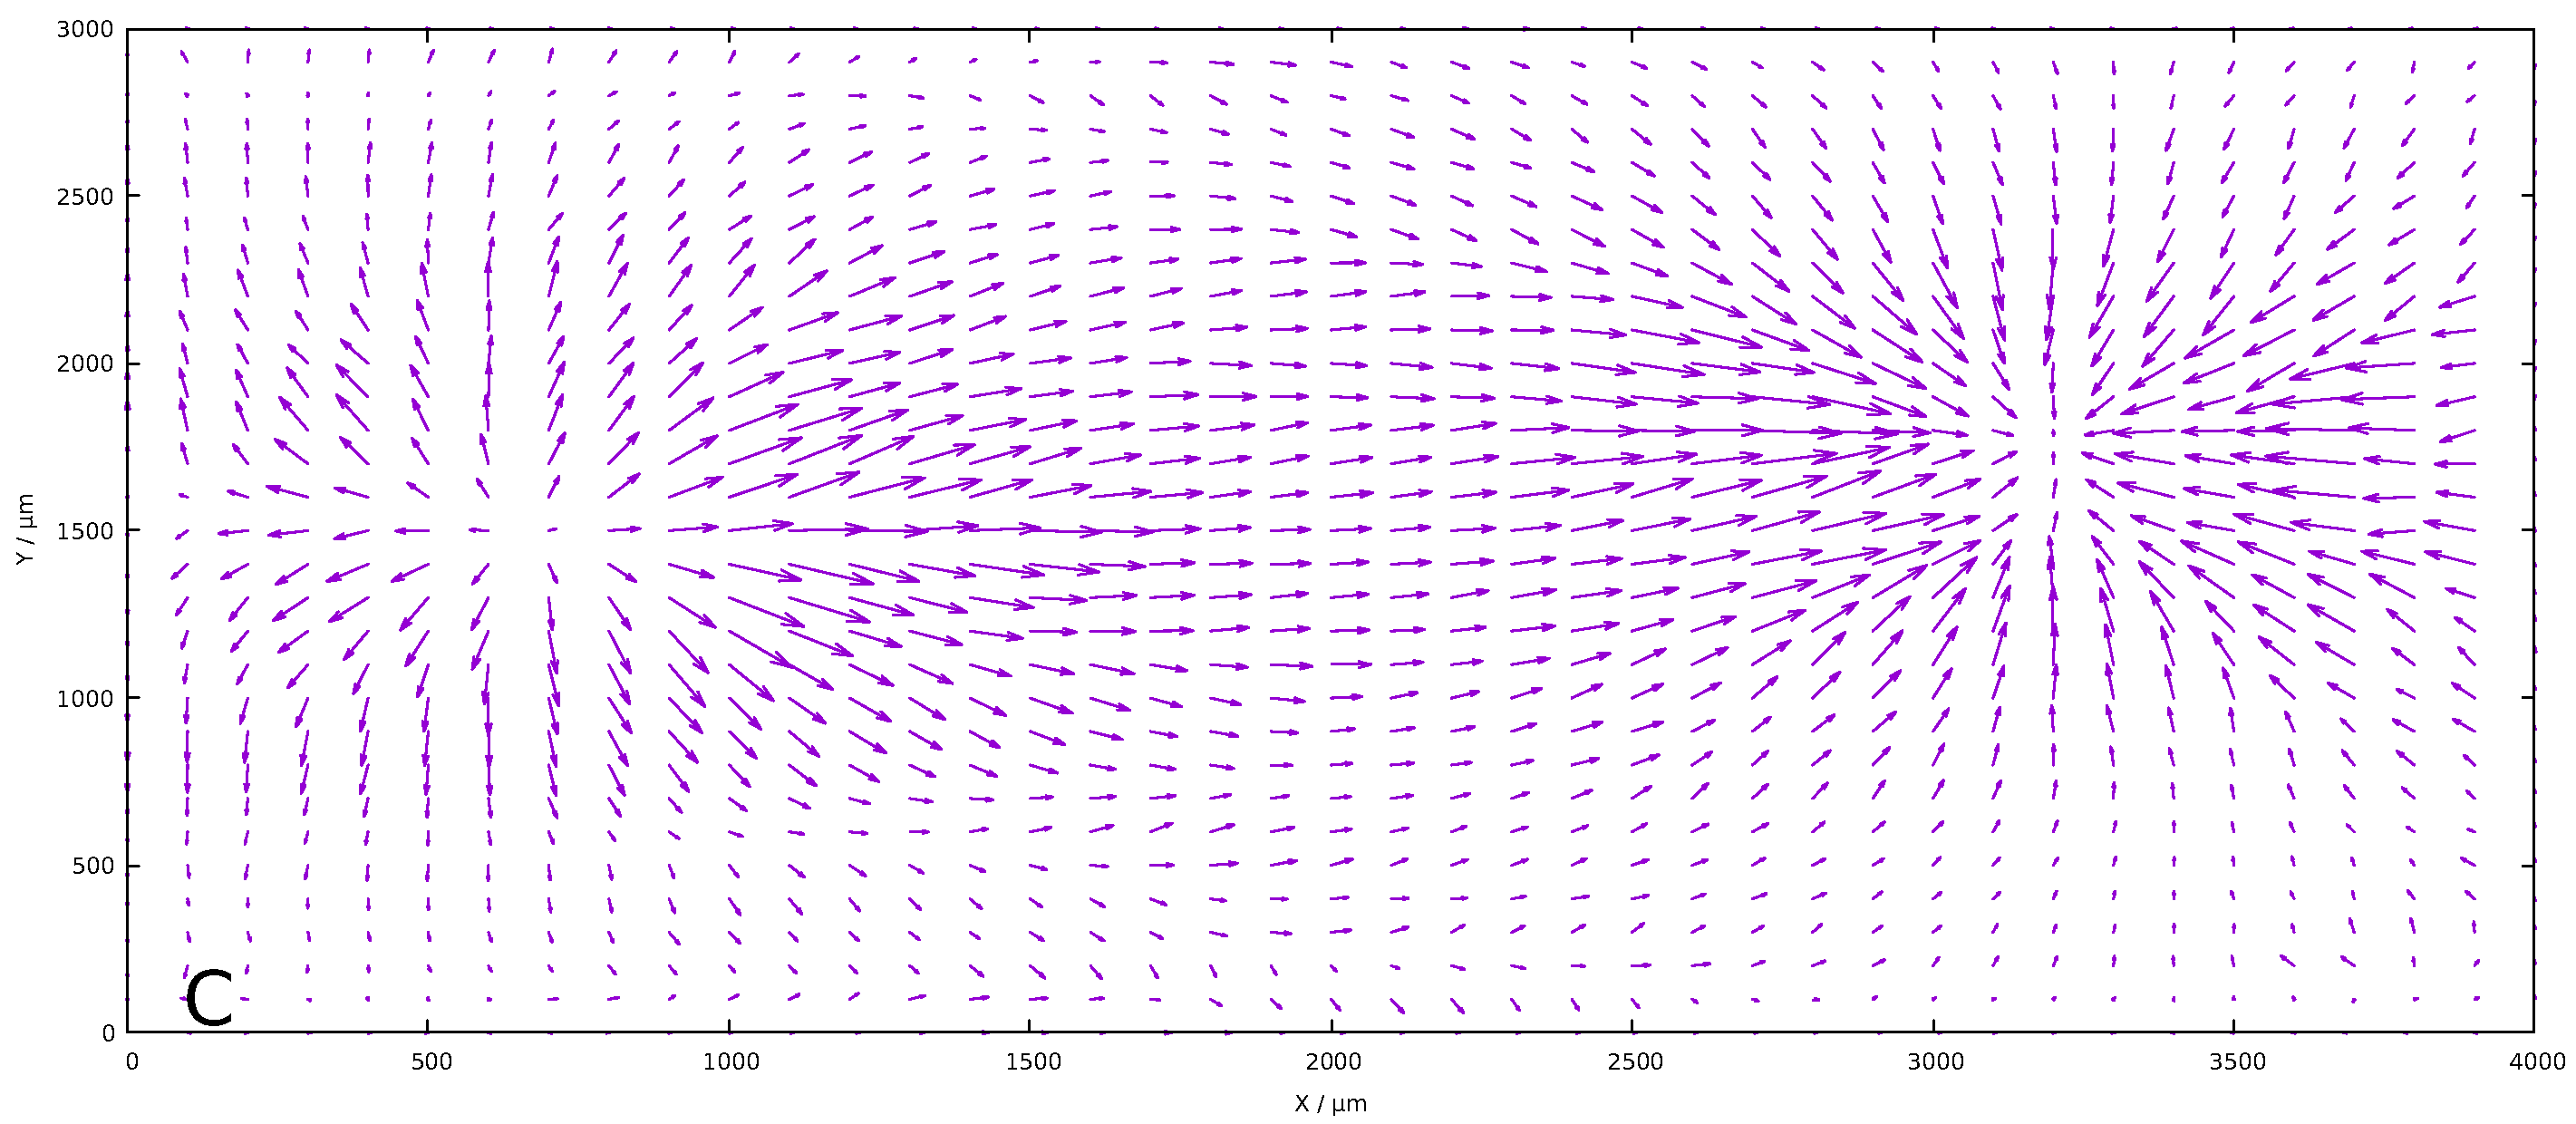
\includegraphics[width=0.8\textwidth]{img/mérések/grafit1_h100.pdf}

\caption{Az említett grafit céltárgyról készült horizontális elektromos mező térképek 100$\upmu$m magasságban mérve}
\label{fig:field_gh}
\end{figure}

\begin{figure}
\centering
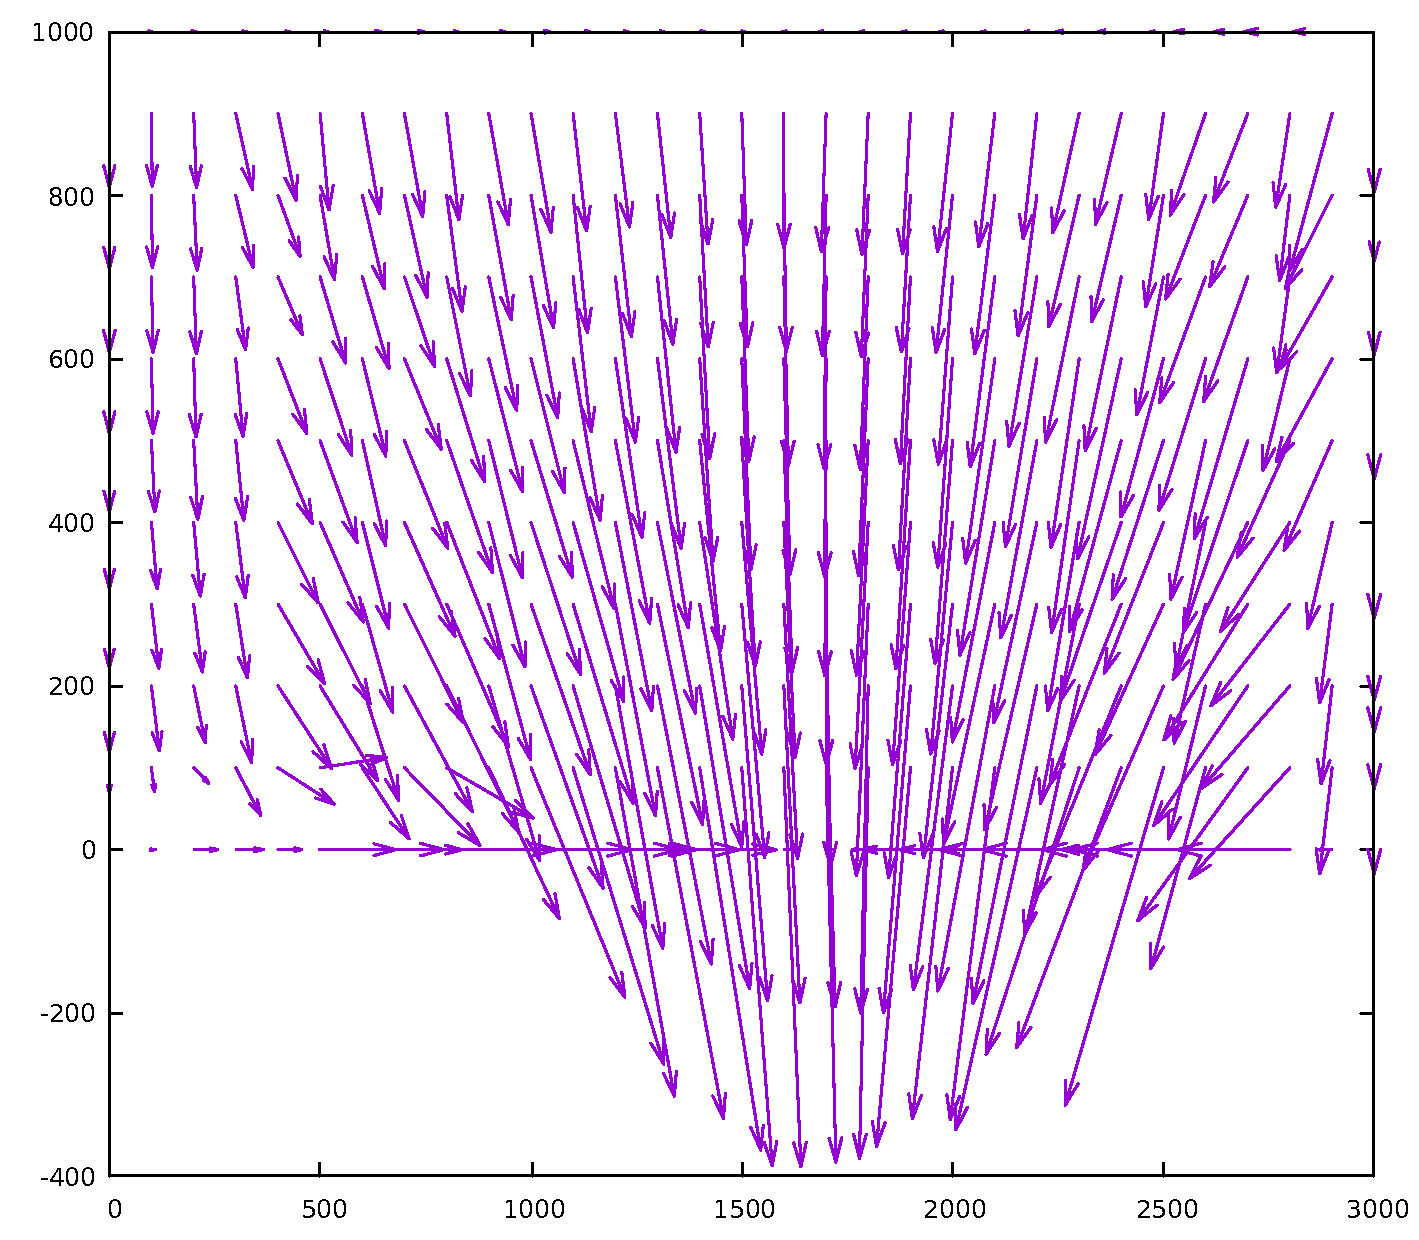
\includegraphics[width=0.8\textwidth]{img/mérések/Fe_v.pdf}
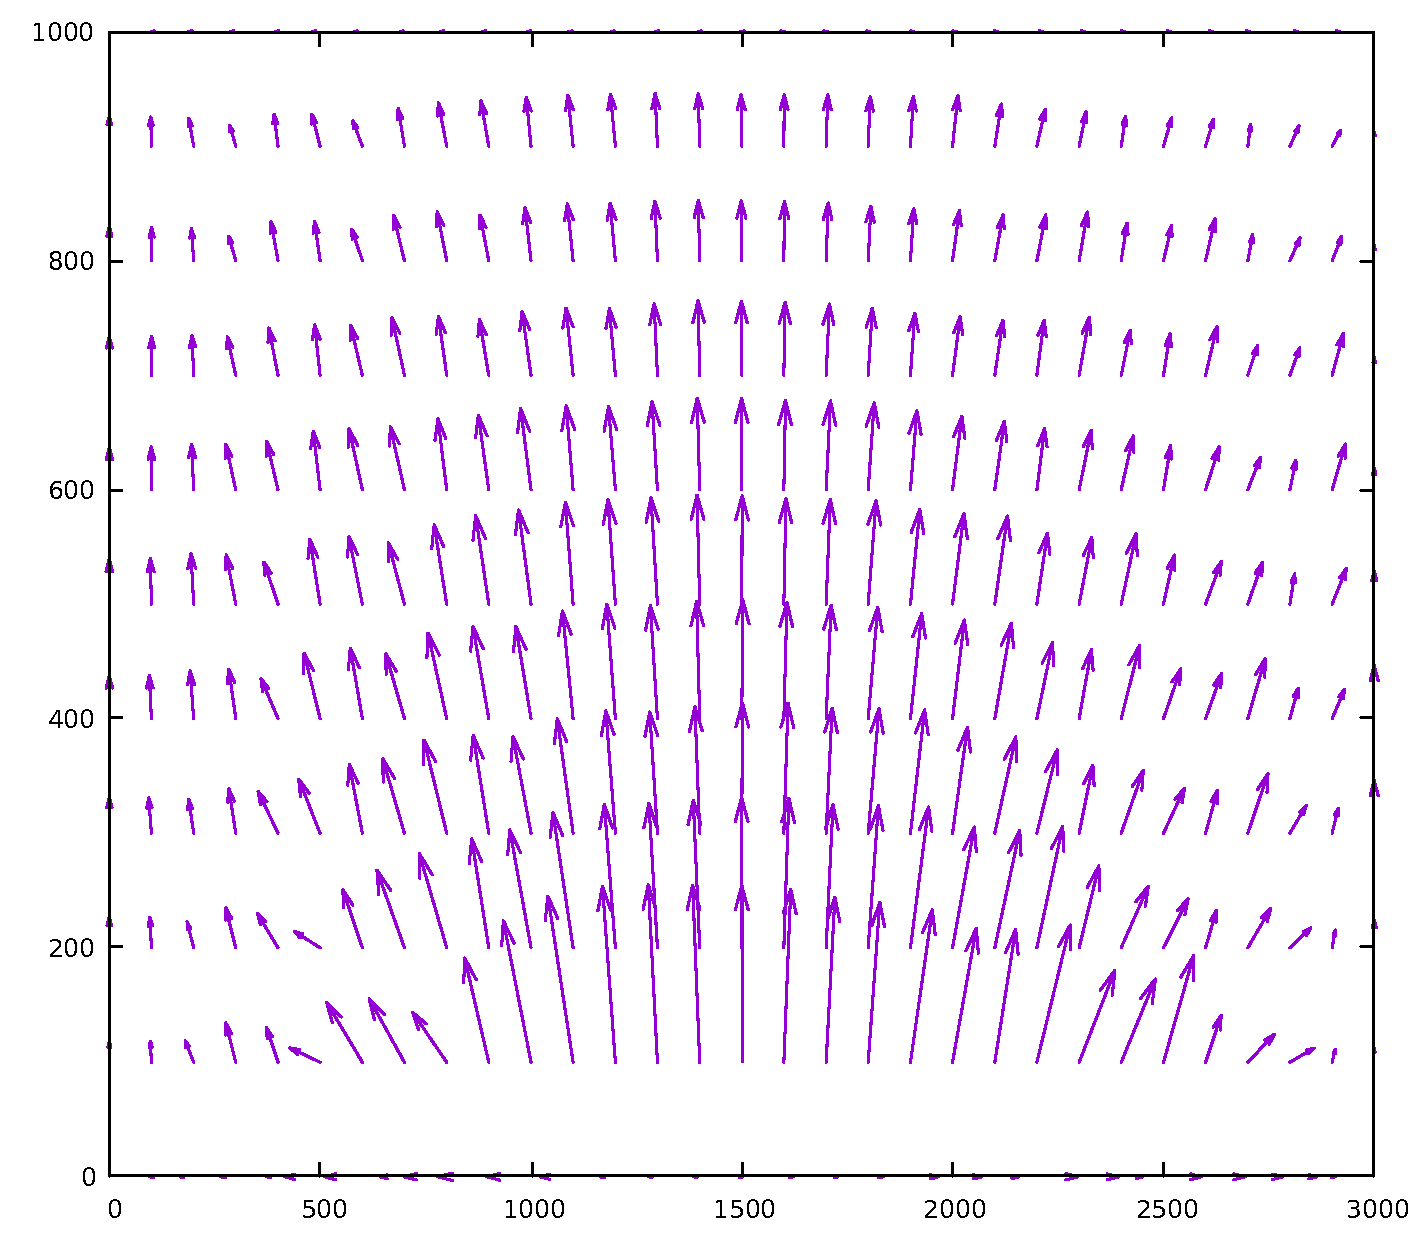
\includegraphics[width=0.8\textwidth]{img/mérések/Zn_v.pdf}
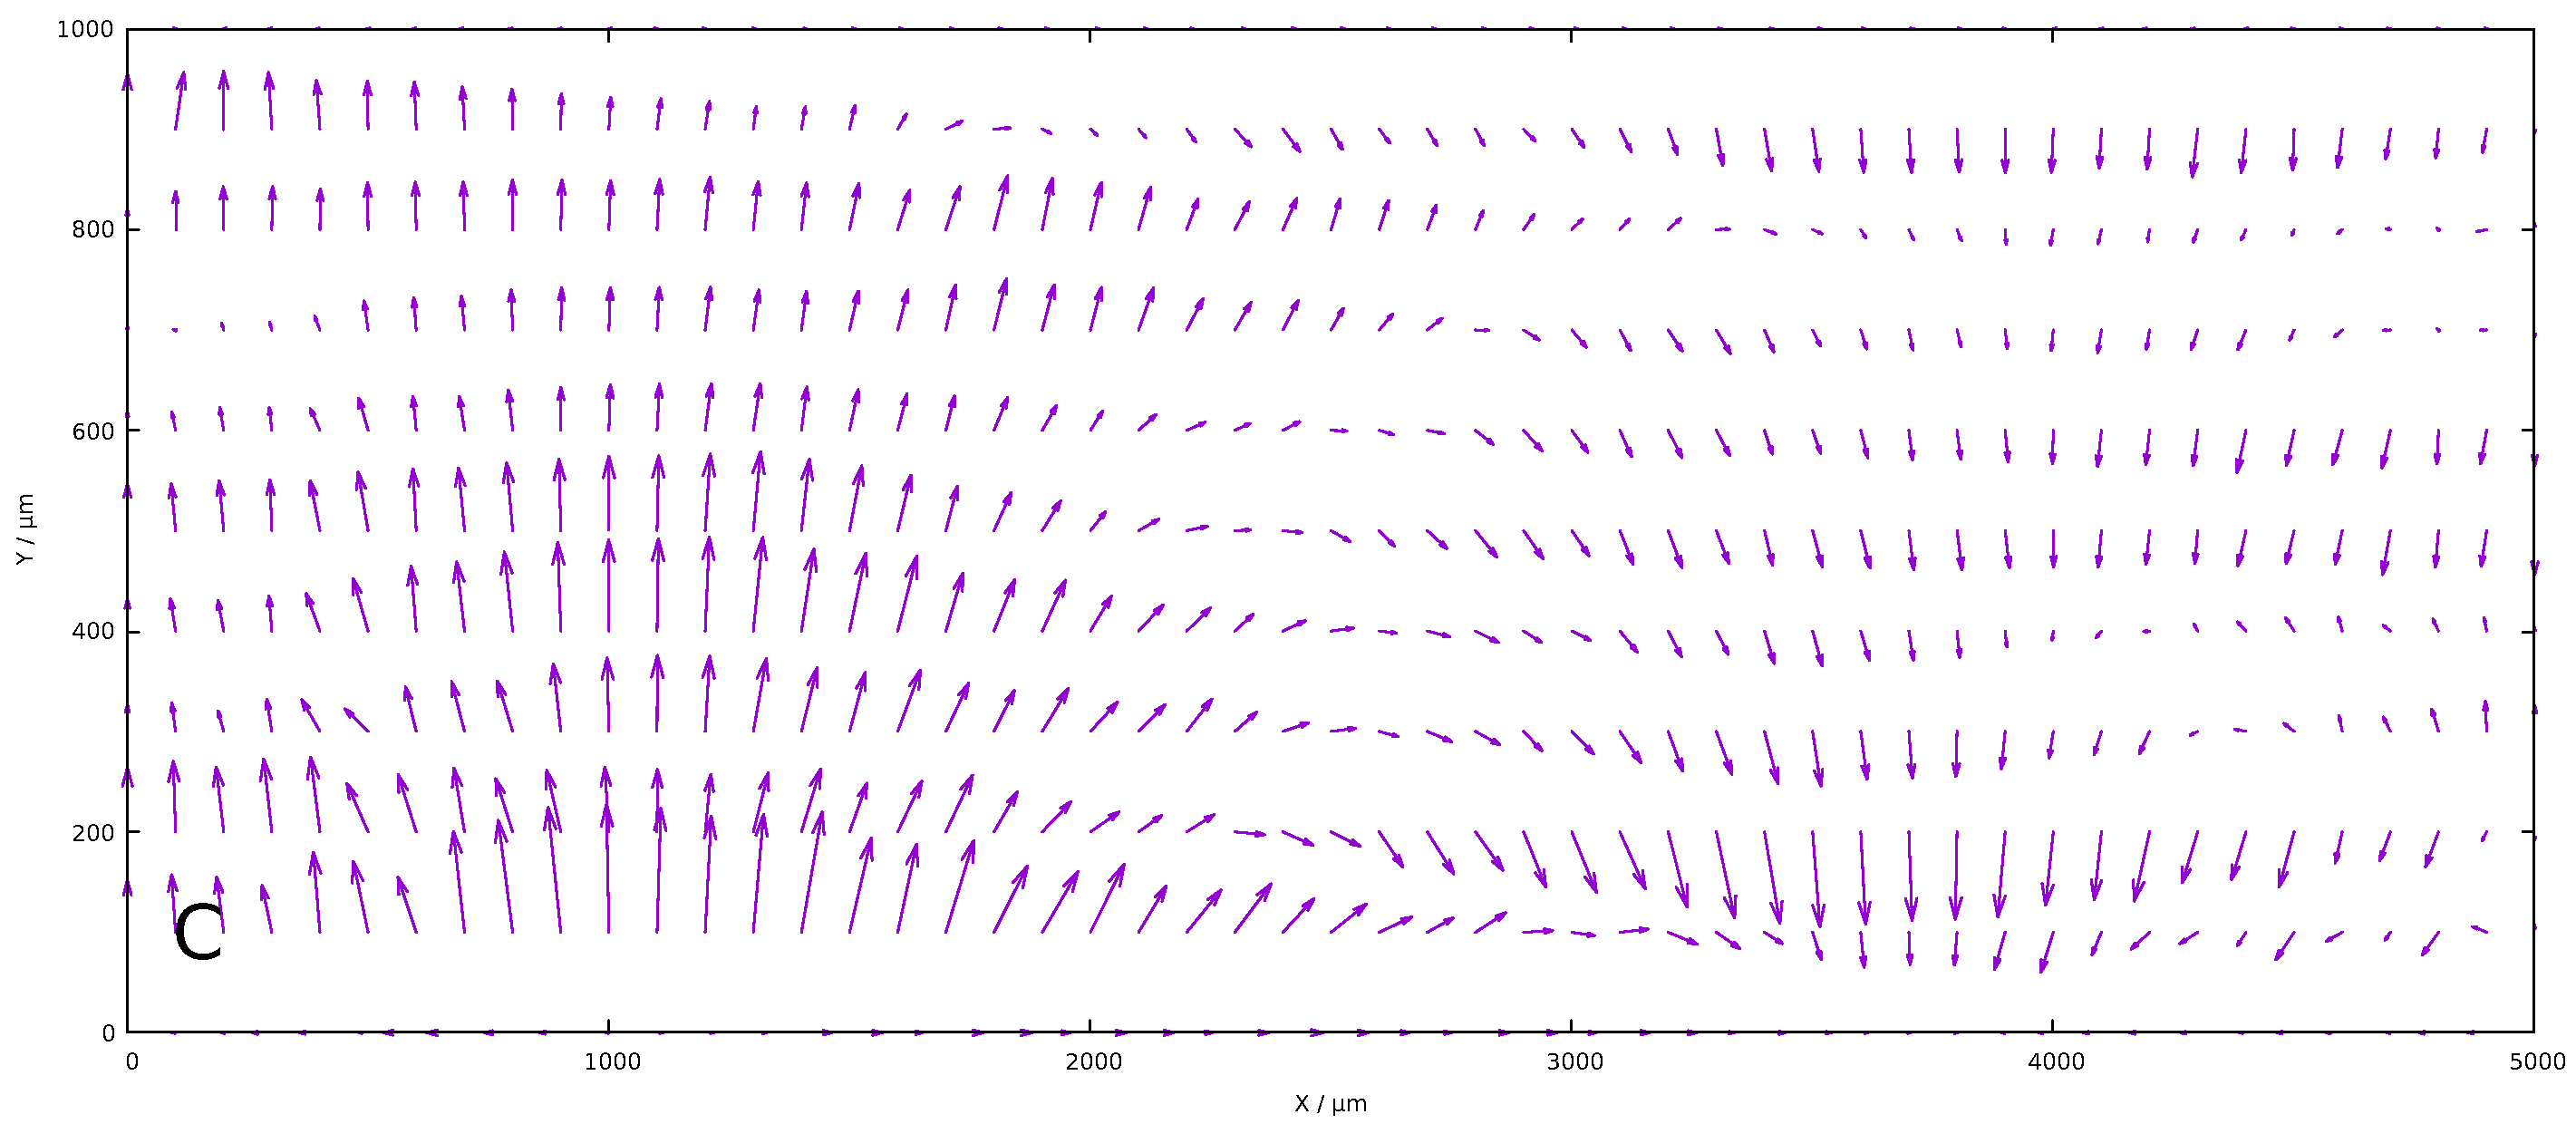
\includegraphics[width=0.8\textwidth]{img/mérések/grafit_v.pdf}

\caption{Az említett céltárgyakról készült vertikális elektromos mező térképek:
(A) a vas katód, (B) a cink anód és (C) a grafit katódja és anódja}
\label{fig:field_v}
\end{figure}

\begin{figure}
\centering
\includegraphics[width=0.5\textwidth, angle=-90]{img/mérések/Fe_h100.eps}
\includegraphics[width=0.5\textwidth, angle=-90]{img/mérések/Zn_h100.eps}
\includegraphics[width=0.5\textwidth, angle=-90]{img/mérések/grafit_h_100.eps}

\caption{Az említett céltárgyakról készült áramsűrűség térképek:
(A) a vas katód, (B) a cink anód és (C) a grafit katódja és anódja}
\label{fig:áramsűrűség}
\end{figure}
